\begin{ledgroupsized}[r]{120mm}
\footnotesize 
\pstart 
\noindent\textbf{\"{U}berlieferung:}
\pend
\end{ledgroupsized} 
\begin{ledgroupsized}[r]{114mm}
\footnotesize 
\pstart \parindent -6mm
\makebox[6mm][l]{\textit{L}}Auszüge mit Bemerkungen aus einem verschollenen Manuskript O. R{\o}mers: LH XXXVII 5 Bl. 216. 1 Bl. 2\textsuperscript{o}. 2 S.
R\"{a}nder ausgefranst mit geringf\"{u}gigem Textverlust.
Textträger durch Papiererhaltungsmaßnehmen stabilisiert.\\%
Cc 2, Nr. 1187
\pend 
\footnotesize 
\pstart
\parindent -6mm
\makebox[6mm][l]{\textit{E}}(Faksimile) \cite{01047}\textsc{O. R{\o}mer}, \title{Korrespondance og afhandlinger}, Kopenhagen 2001, S. 551-555 (Skitser Nr. 13).
\pend
\end{ledgroupsized}
%
%\vspace*{5mm}
%\begin{ledgroup}
%\footnotesize 
%\pstart
%\noindent\footnotesize{\textbf{Datierungsgr\"{u}nde}: Von Leibniz selbst datiert, obere linke Ecke.}
%\pend
%\end{ledgroup}
%
\vspace{8mm}
\pstart%
\normalsize%
\noindent%
%[216~r\textsuperscript{o}]
[216~r\textsuperscript{o}] 
Xb. 1675 extraxi ex eius Mso.
\pend
\count\Afootins=1200
\count\Bfootins=1200
\count\Cfootins=1200
\pstart%
\noindent%
Propositionum \protect\index{Namensregister}{\textso{R{\o}mer}, Ole 1644-1710}\edtext{R\"{o}meri}{\lemma{}\Bfootnote{R\"{o}meri \textit{erg. L}}} Mechanicarum circa rotas dentatas\protect\index{Sachverzeichnis}{rota dentata} \edtext{pars 2\textsuperscript{da}}{\lemma{}\Afootnote{\textit{Unterhalb} pars 2\textsuperscript{da}: Non vidi ejus partem primam.\vspace{-8mm}}} de curvis quibusdam pro figura dentium:
\pend
\vspace{1em}% PR: Rein provisorisch !!!
\pstart
\centering
\noindent
% \begin{wrapfigure}{l}{0.4\textwidth}
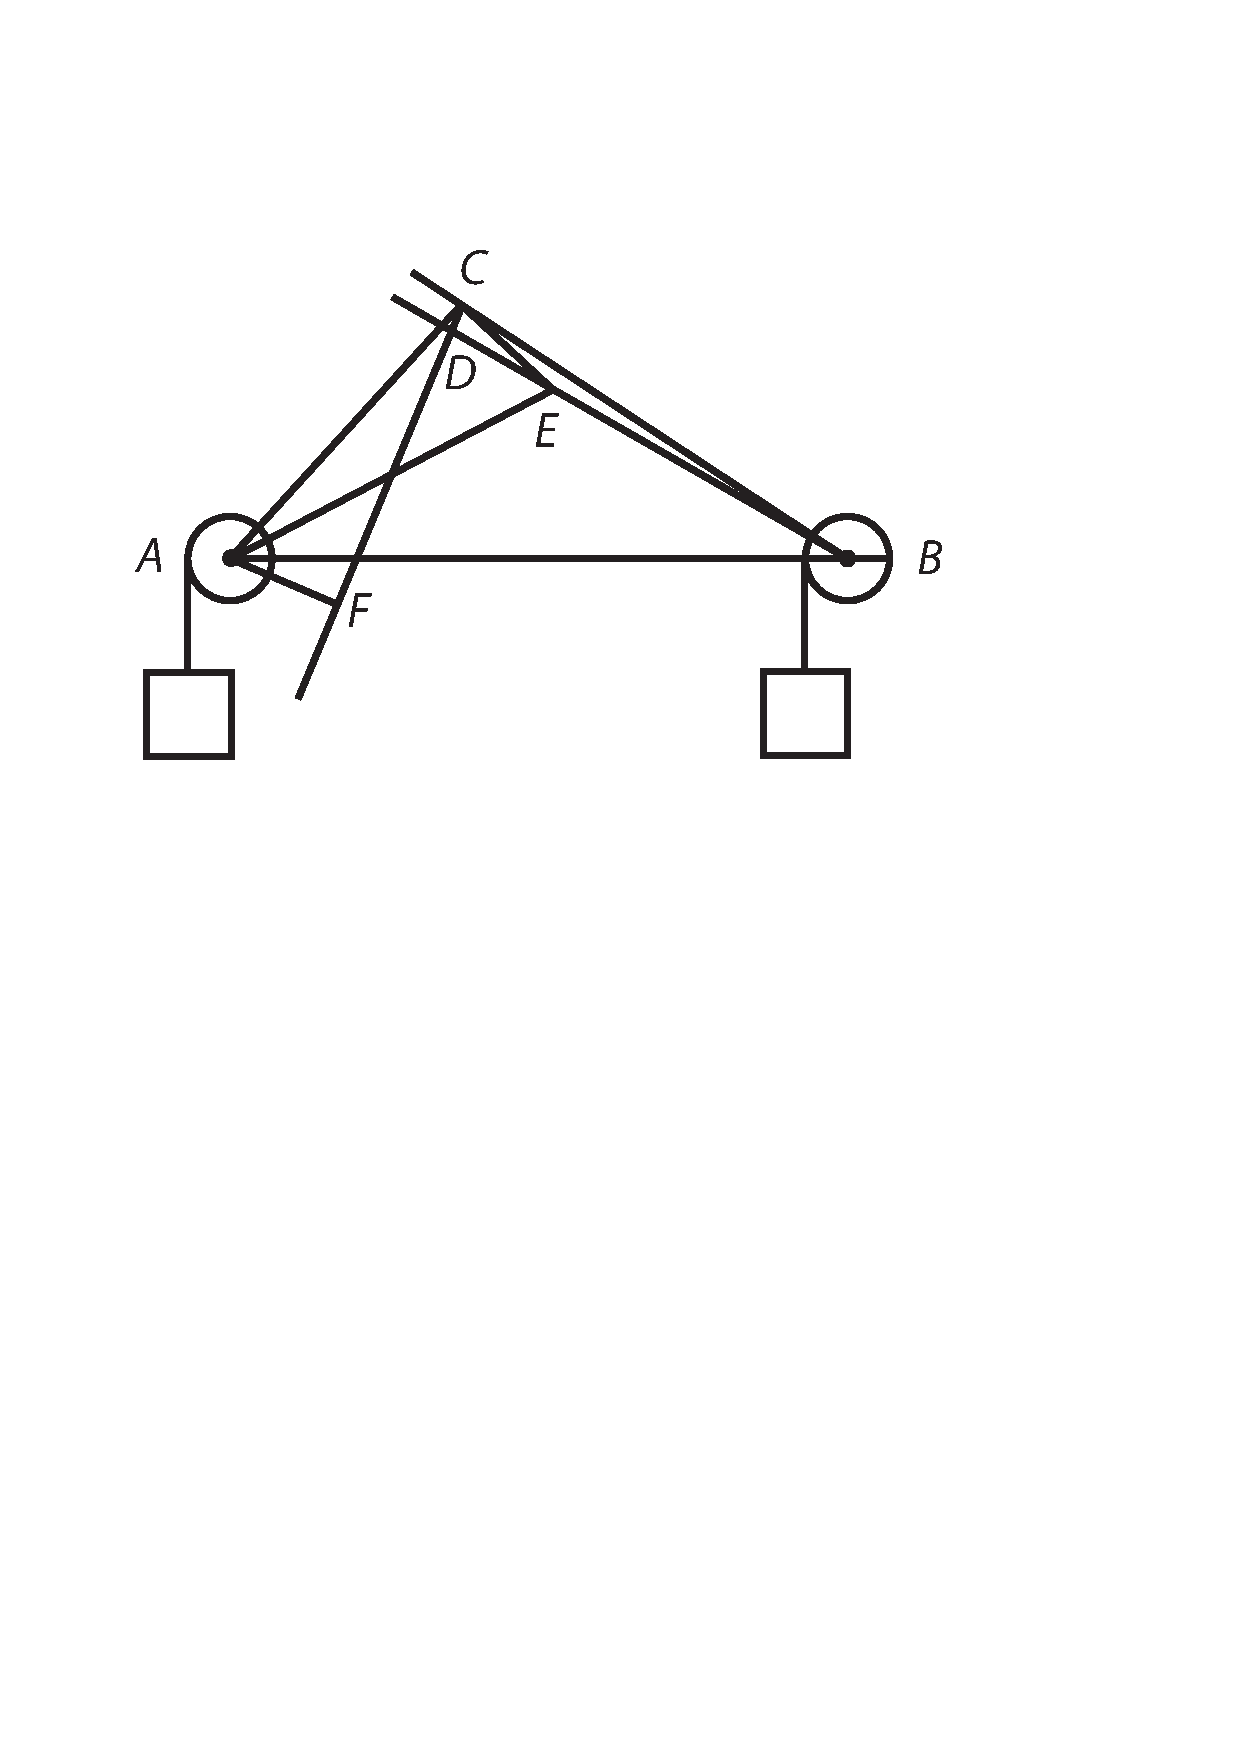
\includegraphics[width=0.48\textwidth]{images/LH03705_216r-d1.pdf}\\
\centering[\textit{Fig. 1}]
% \end{wrapfigure}
\pend
\vspace{1em}% PR: Rein provisorisch !!!
\pstart 
\noindent
\textso{Prop. 1.}
\setline{11}Aequalibus ponderibus se urgeant rotae $A$, et $B$.
Premat moveatque radius $BC$, radium $CA$ ut punctum contactus $C$ proximo momento sit in $E$.
Dico motum radii $CB$ qui est angulus $CBE$ esse ad motum radii $AC$, qui est angulus $CAE$ ut dictorum radiorum vires. Nam vires ex prioribus, inquit, sunt ut $CB$ ad $AF$ (+ non dicit qualis sit $CF$ +). Quod si ergo ostendimus angulum $CAE$, esse eodem modo ad angulum $CBE$, ostendemus\hfill vires\hfill esse\hfill ut\hfill hos\hfill angulos.\hfill
Suppono\hfill dictos\hfill arcus\hfill \edtext{[tam]}{\lemma{tum}\Bfootnote{\textit{L ändert Hrsg.}}}\hfill parvos\hfill ut\hfill censeri\hfill possint 
\pend
\newpage
\pstart
\noindent rectae, erunt $CDE$, et $ACE$ anguli recti adeoque triangula $CDE$, $CAF$ (: enuntiari deberet $AFC$ :) \edtext{similia. Hinc}{\lemma{similia.}\Bfootnote{\textit{(1)}\ Ergo $\displaystyle\frac{CD}{CE} \sqcap \frac{AC}{AF}$ \textit{(2)}\ Hinc \textit{L}}} sequens inquit ratiocinium[:]
\pend
\vspace{0.5em}% PR: Rein provisorisch !!!
\pstart
\noindent%
$\begin{array}{ccl}
\overbrace{CAE\text{ est ad } CBD}^{\displaystyle\text{ratio angulorum parvorum}}&\text{ut \textit{CB} ad \textit{AC}}&\hspace*{6mm}+\text{\textit{CE} ad \textit{DC}} \\
\underbrace{CB\text{ est ad }AF}_{\displaystyle\text{ratio virium}}&\text{ut \textit{CB} {ad\reversemarginpar\marginnote{\scriptsize\hspace{-13mm}5}} \textit{AC}}&\underbrace{+\text{\textit{AC} ad \textit{AF}}}_{\displaystyle \sqcap\ \text{rationi \textit{CE} ad \textit{CD}}}\\
\end{array}$
\pend
\vspace*{0.5em}% PR: Rein provisorisch !!!
\pstart%
\noindent%
Ergo \setline{7}eadem ratio angulorum parvorum quae virium (+ ipse non probat haec quae assumit ob similitudinem $\bigtriangledown$\textsuperscript{lorum} $ACF$. $CED$ sed res nobis aliunde nota +). Scilicet ponit \edtext{perpendicularem ad contactum, transire}{\lemma{perpendicularem}\Bfootnote{\textit{(1)}\ transire \textit{(2)}\ ad contactum, transire \textit{L}}} per alterutrius rotae centrum. Intelligit credo $CF$ transire per $A$ quicquid sit ista non habent opus demonstratione. Nam per se patet tantam esse vim quanta est quantitas motus, quae est ut particulae revolutionum seu anguli.
\pend
\vspace{1.5em}
\pstart
\centering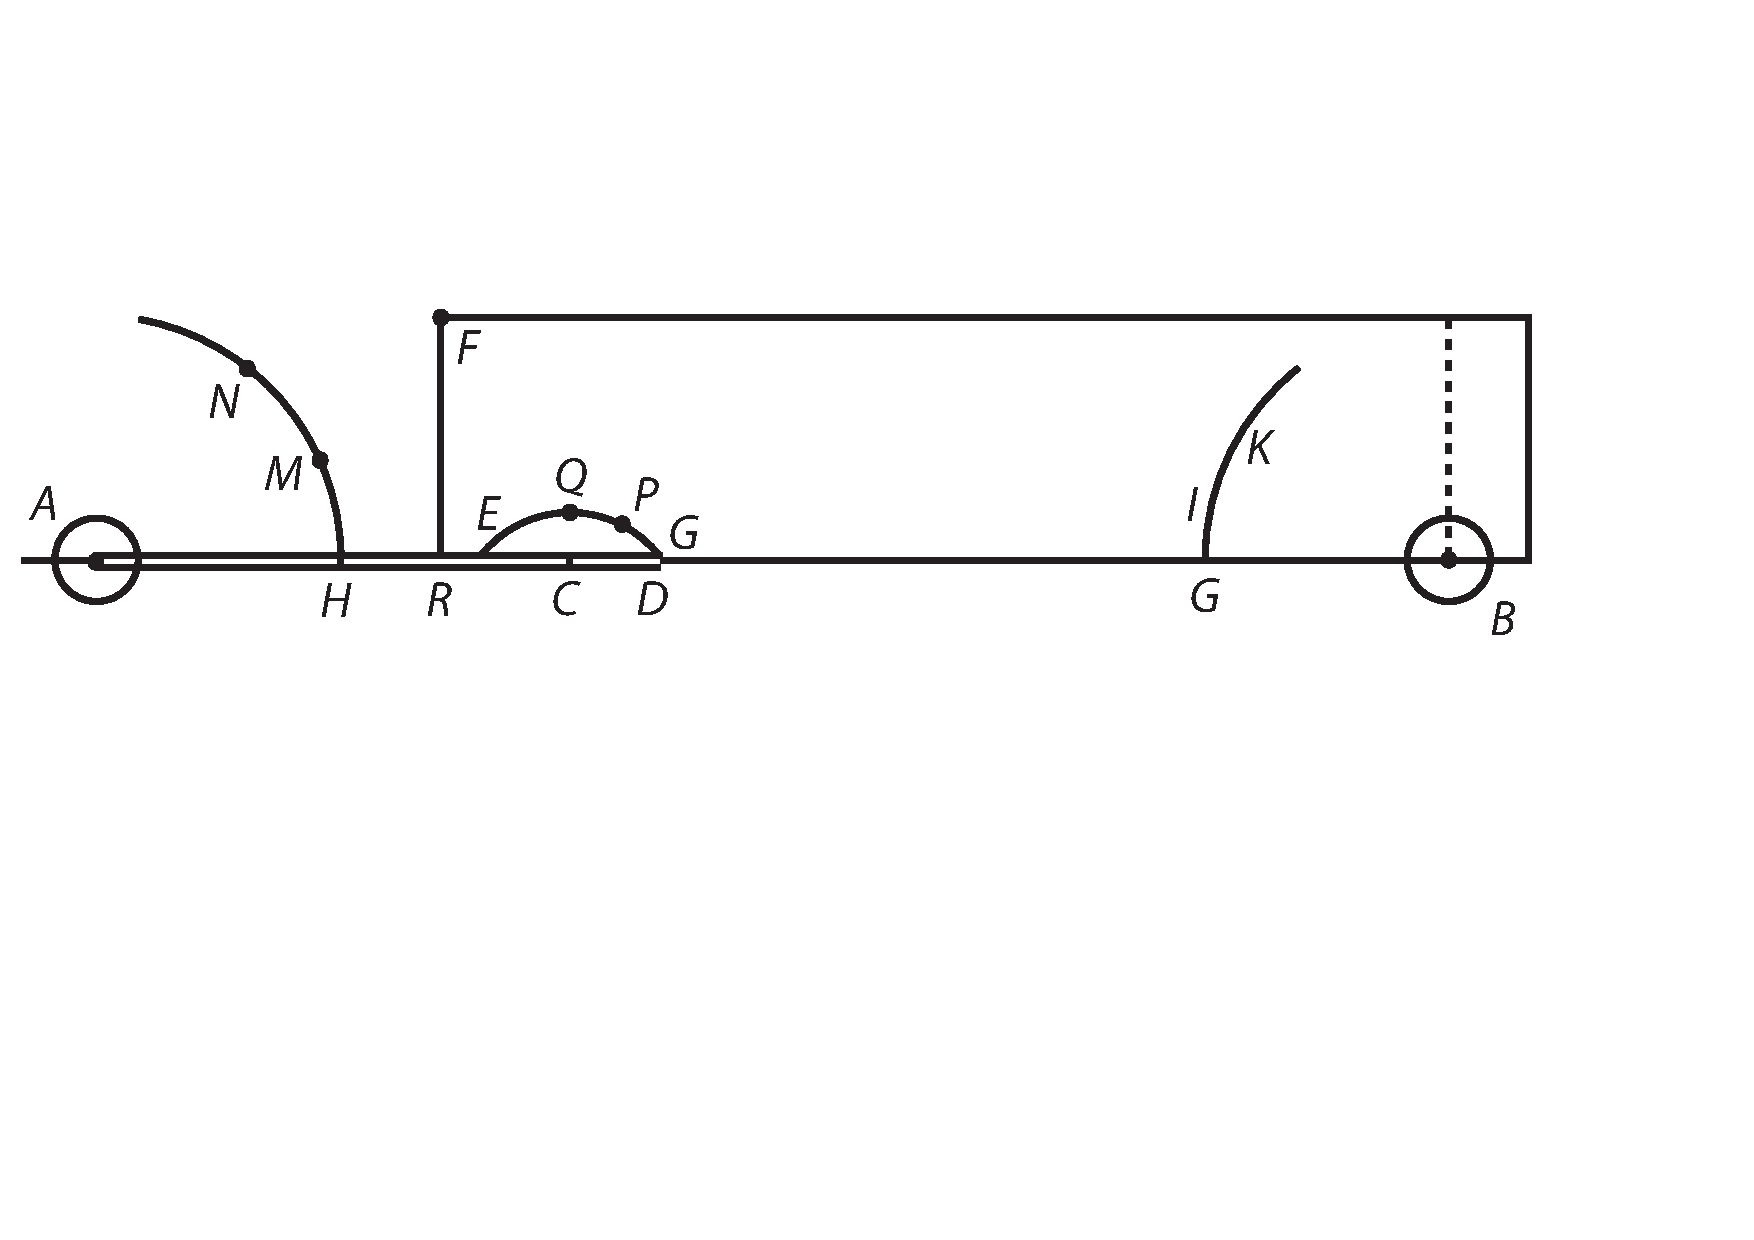
\includegraphics[width=0.9\textwidth]{images/LH03705_216r-d2.pdf}\\
\centering%
[\textit{Fig. 2}]%
\edtext{}{\lemma{\hspace*{1,9mm}[\textit{Fig. 2}]}\killnumber\Afootnote{%
\textit{Leibniz streicht das $G$ nahe $B$ und notiert am Rand:} Pro $G$ hic alia esse deberet litera.\vspace{-4mm}}} 
\pend 
\vspace{1.5em}
\pstart Sit \setline{13}$AC$ ad $CB$, \edtext{qualiscunque verbi gratia}{\lemma{}\Bfootnote{qualiscunque verbi gratia \textit{erg. L}}} ut 1. ad 3. Sit $AD$ major $AC$. Sit radius $AD$ mobilis circa centrum $A$, et totum planum $BRF$ mobile circa centrum $B$ omnia in eodem plano. Moveatur \edtext{Radius $AHD$ ita ut}{\lemma{$AHD$}\Bfootnote{\textit{(1)}\ circa \textit{(2)}\ in area \textit{(3)}\ ita ut \textit{L}}} punctum $H$ sumtu pro arbitrio in $AD$; describat arcum $HM$. Eodem tempore moveatur planum $BRF$, a $G$ in $I$ circa [centrum]\edtext{}{\Bfootnote{radium\textit{\ L \"{a}ndert Hrsg.}}} $B$, ut sumto $BG \sqcap AH$, sit $GI$ ad $HM$, in ratione aliqua data, ut v.g. $AC$ ad $CB$ seu ut 1. ad 3. Notetur punctum $P$, in plano quo radius $AHD$, cum ex $H$ pervenit in $M$, et cum eodem tempore planum pervenit \edtext{in $I$, sua extremitate}{\lemma{in $I$,}\Bfootnote{\textit{(1)}\ puncto $I$ \textit{(2)}\ sua extremitate \textit{L}}} $D$, in plano reperitur. Si stylum ponamus in $D$, designa$\langle$bit$\rangle$ in plano punctum $P$. Eodem modo puncto $H$ veniente in $N$, et puncto $G$ in $K$, stylus $D$, notabit $Q$. Quo facto designabitur curva $GPQ$ quae erit talis, ut eadem semp$\langle$er$\rangle$ vi polleat radius AD. Nam si dens jam seu vectis unus sit $AD$, alius $BGPQ$ patet ita duci unum ab alio in curva, ut eadem sit semper ratio \edtext{revolutionum. Ideoque et}{\lemma{revolutionum.}\Bfootnote{\textit{(1)}\ Et \textit{(2)}\ Ideoque et \textit{L}}} vis. 
\pend 
\pstart \edtext{Si ponamus curvam non describi in plano mobili sed contra planum quale erat $BFR$ esse immobile,
et loco quod planum ibat de $R$ versus $F$ contra ibit tota machina $ADB$ circa $B$ retro deorsum seu ab $F$ ad $R$
et interim movebitur $D$ punctum describens circa centrum $A$, in arcu $HMN$ eadem qua ante proportione,
et patet eandem quae ante describi curvam.}%
{\lemma{Si ponamus}\Bfootnote{[...] centrum $A$, in \textit{(1)}\ radio $P$ \textit{(2)}\ arcu $HMN$ eadem [...] describi curvam. \textit{erg. L}}}
\pend 
\vspace{1.5em}
\pstart
\centering
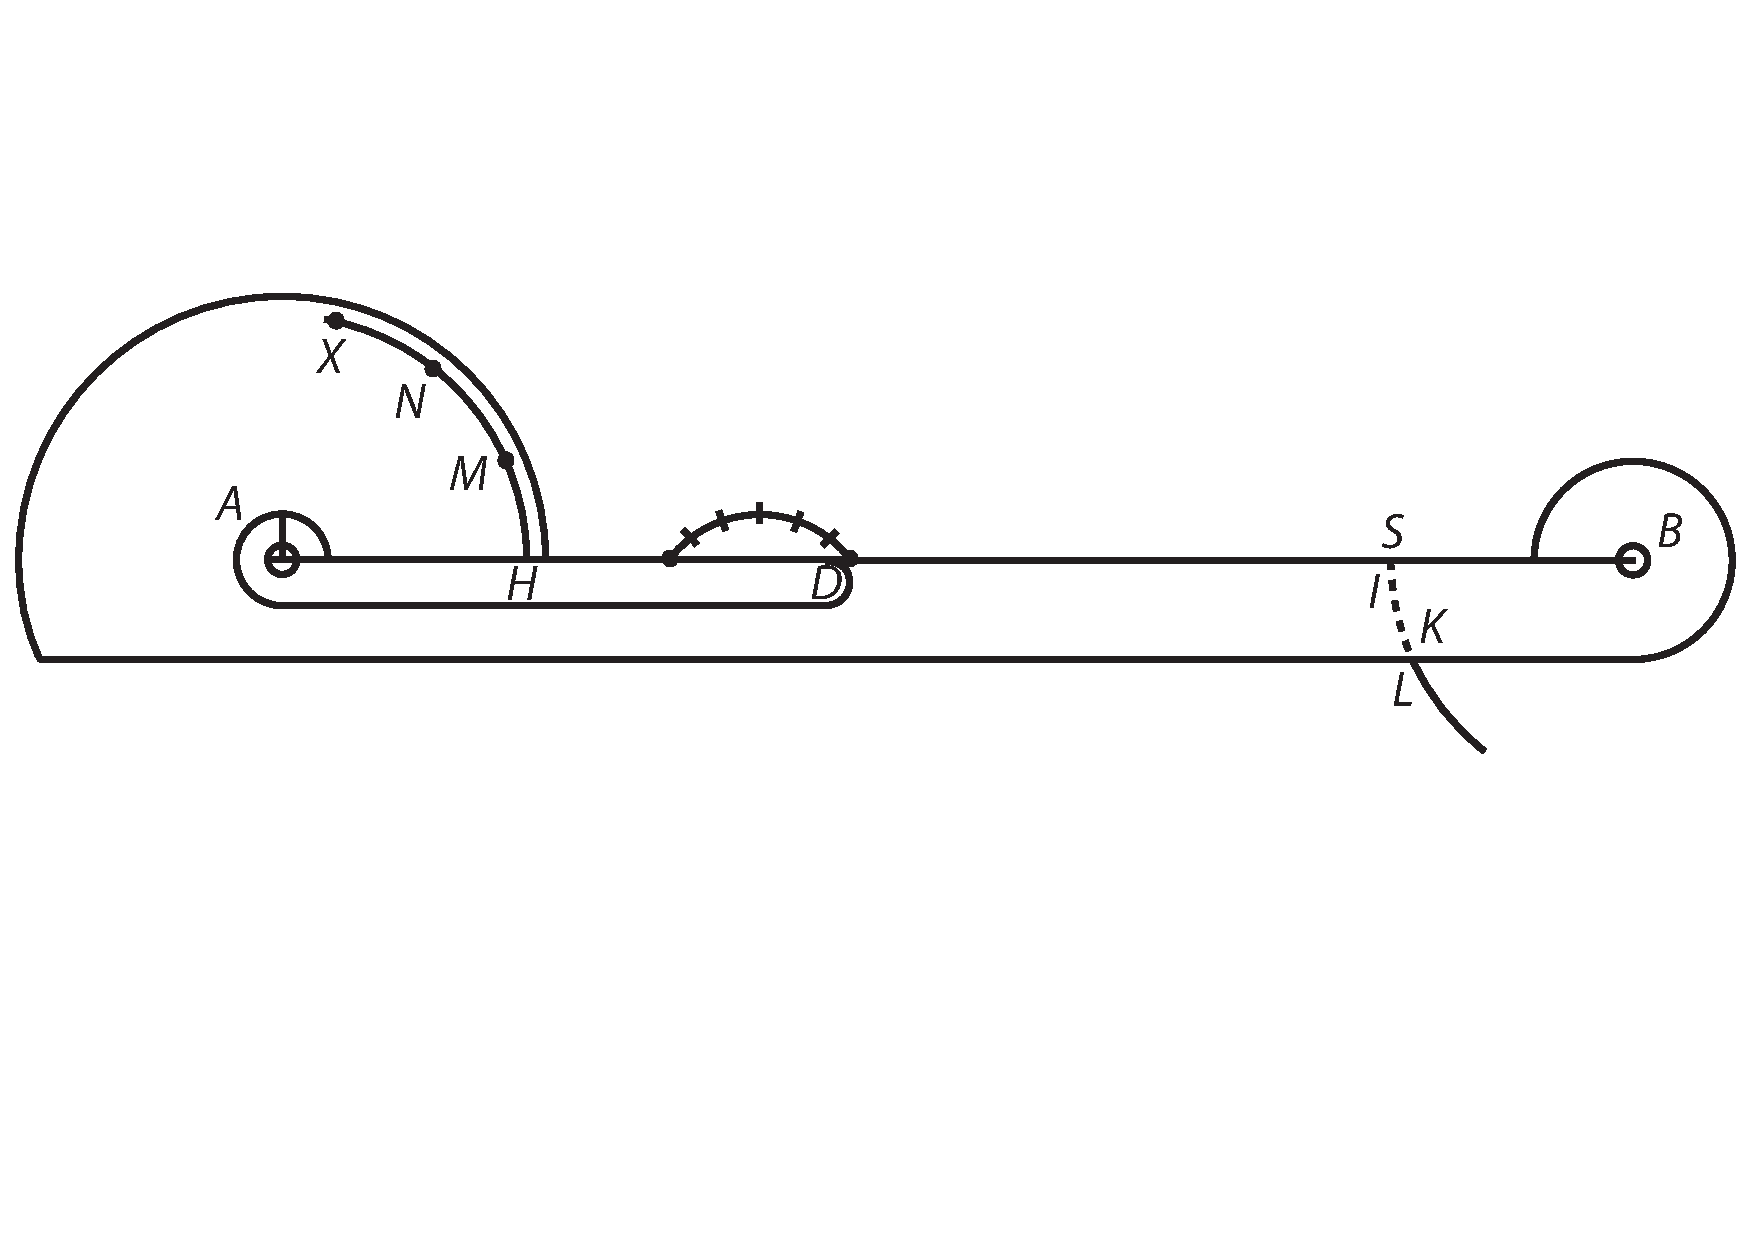
\includegraphics[width=0.92\textwidth]{images/LH03705_216r-d3.pdf}\\
\centering[\textit{Fig. 3}]
\pend
\vspace{1.5em}
\pstart Prior \setline{12}delineandi modus inventum prodidit, posteriorem ait ad investigandas proprietates videri accommodatiorem. In primis ad inveniendas curvae tangentes, quem in finem lemmata. Lemma primum: Si super plano $ABC$ punctum $A$ moveatur in linea $AB$ motu aequabili, et planum $A$, interim feratur super alio plano $FG$, motu etiam aequabili, ratioque spatiorum confectorum sit ut $AB$ ad $AC$, dico punctum $A$, ferri in linea $AD$ diagonali, et per consequens lineam $BC$ bisectam in $E$ monstrare punctum $E$ per quod revera \edtext{tendit punctum}{\lemma{tendit}\Bfootnote{\textit{(1)}\ curva \textit{(2)}\ punctum. \textit{L}}}. 
\pend 
\newpage
\pstart
\noindent
\hspace{4mm}
\begin{minipage}[t]{0.5\textwidth}
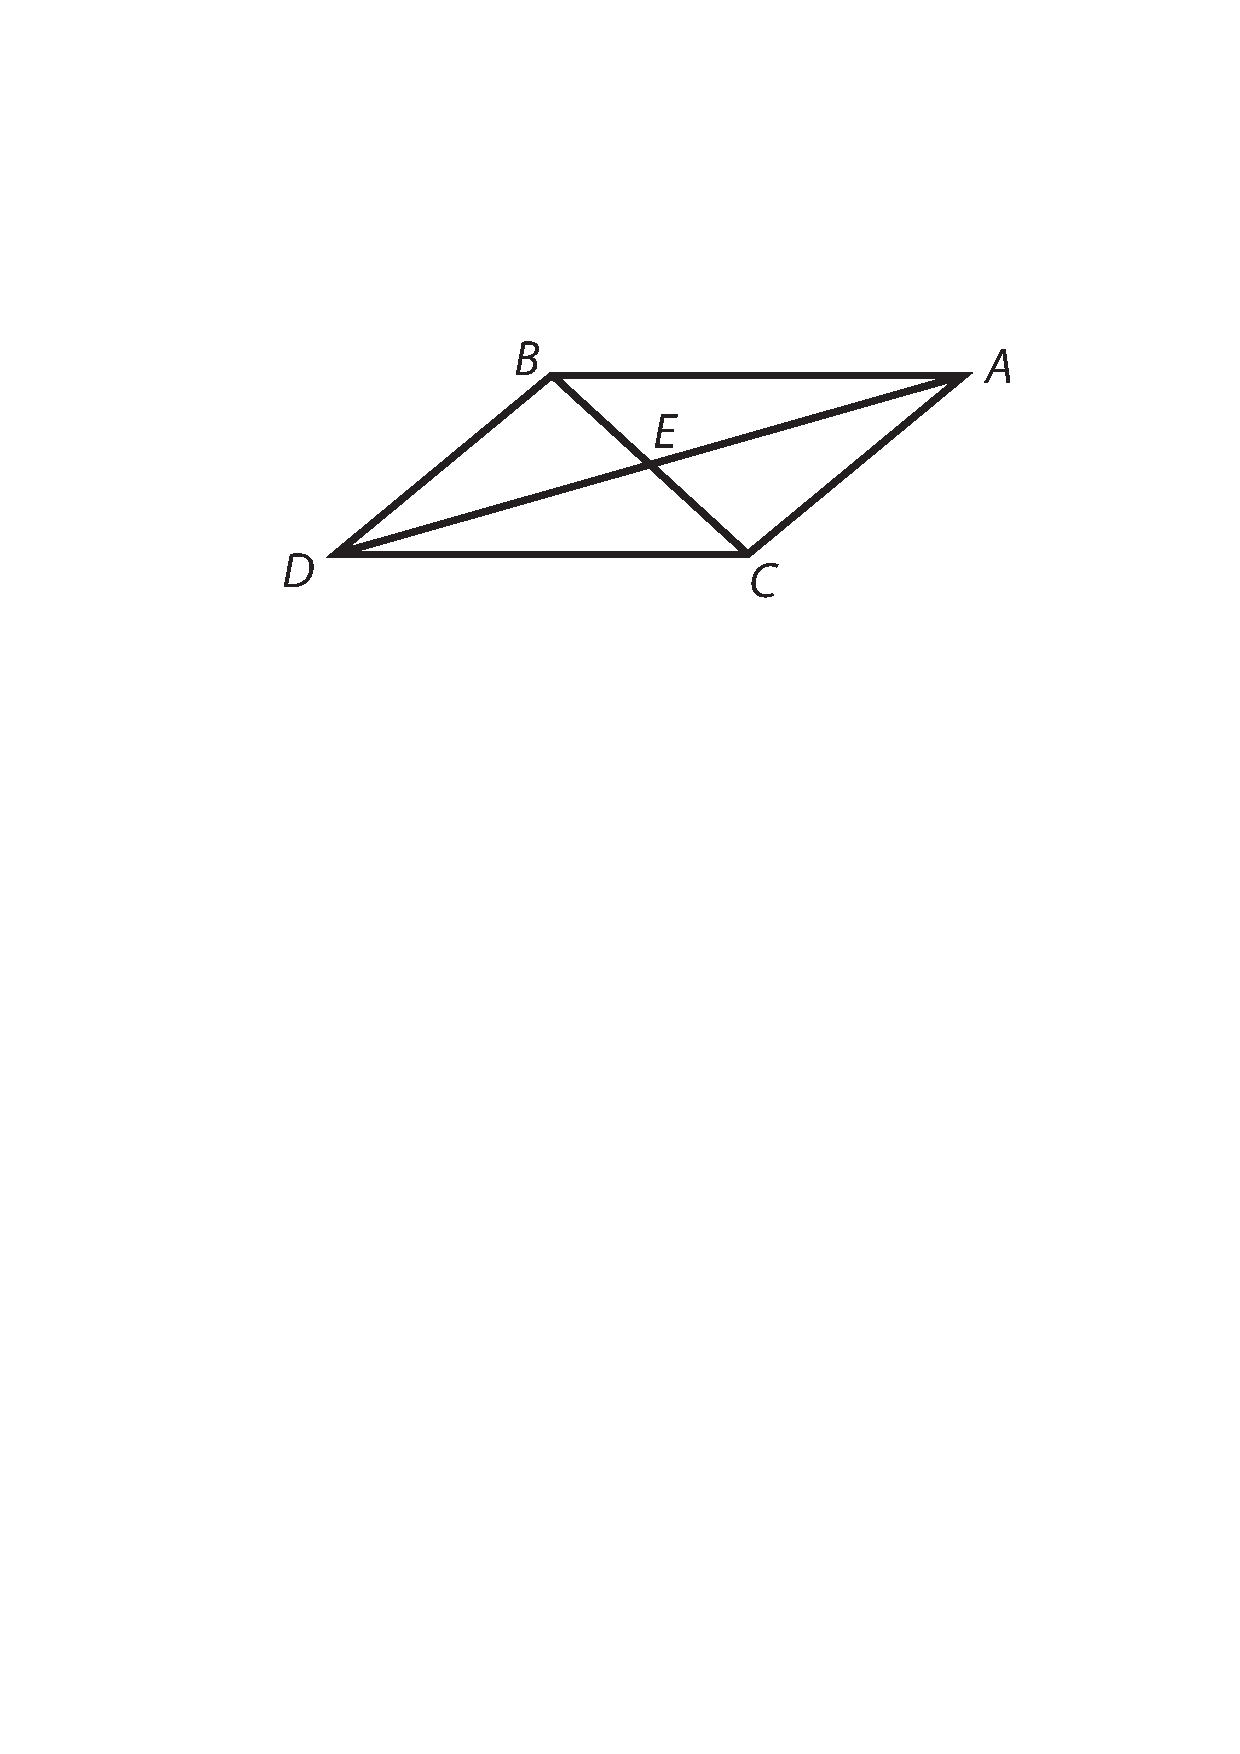
\includegraphics[width=0.9\textwidth]{images/LH03705_216r-d4.pdf}
\end{minipage}
%\hspace*{13,3mm}
\begin{minipage}[t]{0.5\textwidth}
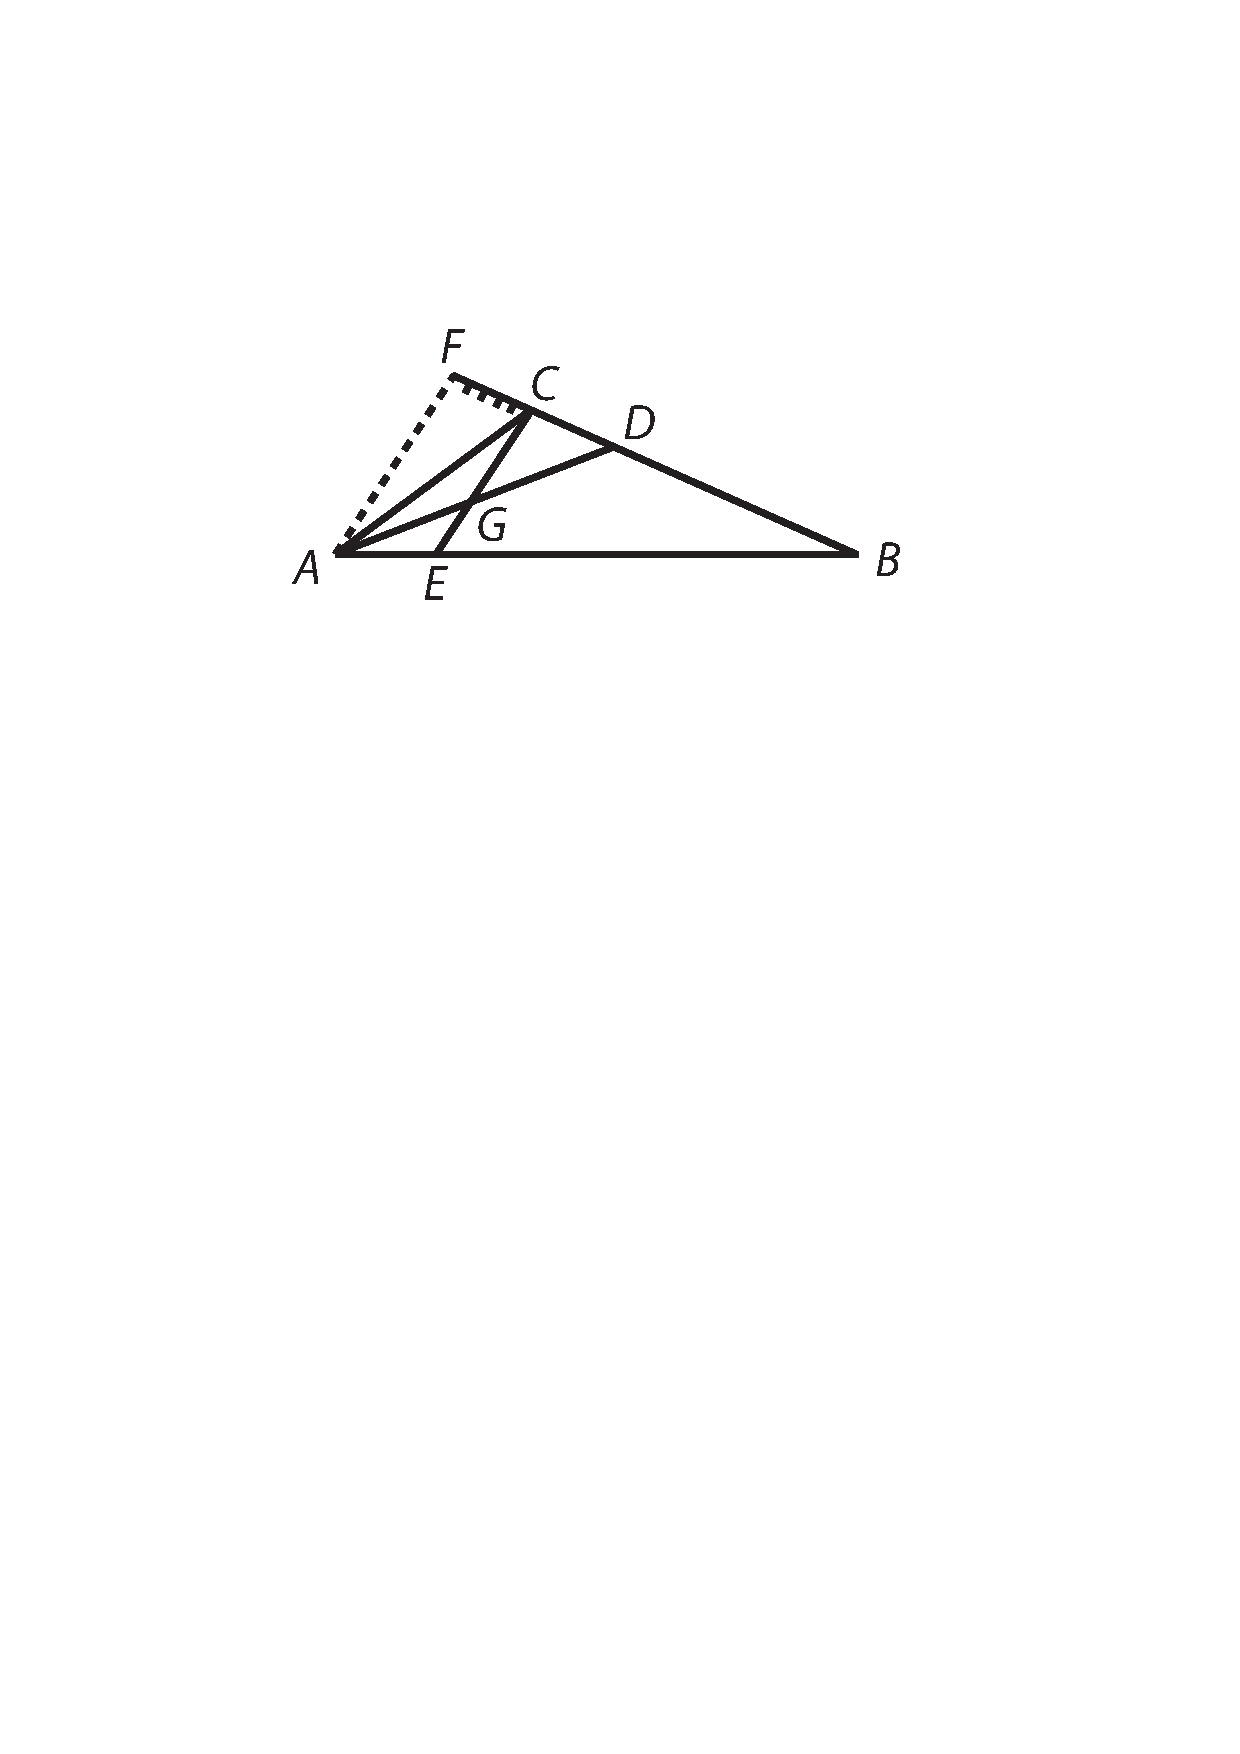
\includegraphics[width=0.76\textwidth]{images/LH03705_216r-d5.pdf}\\
\end{minipage}
%\vspace*{4mm}
\hspace*{25mm} [\textit{Fig. 4}]\hspace*{54mm} [\textit{Fig. 5}]
\pend
\vspace{2em}
\pstart Lemma \setline{1}alterum: Si in $\bigtriangledown$\textsuperscript{lo} $ABC$, ab $A$ ducatur quaelibet $AD$, quae secetur bifariam in $G$, a linea $CGE$, erit ut $CD$ \edtext{ad $BC$, ita $AE$}{\lemma{ad $BC$}\Bfootnote{%
\textbar\ ita \textit{streicht Hrsg.} \textbar\ , ita $AE$ \textit{L}}} ad $EB$. Nam producta $BC$ in $F$ et facto $FC$, aequali ipsi $CD$, erunt ob aequalitatem segmentorum $AG$, $GD$; item $CD$, $FC$, lineae $AF$, et $EC$ parallelae, et per consequens ut $FC$, \edtext{seu $CD$, ad $CB$}{\lemma{seu $CD$,}\Bfootnote{\textit{(1)}\ sic $AE$ \textit{(2)}\ ad $DB$ \textit{(3)}\ ad $CB$ \textit{L}}} sic $AE$ ad $EB$. 
\pend 
\count\Afootins=1500
\count\Bfootins=1500
\count\Cfootins=1500
\pstart His ita praemissis curvae tangens determinatur: ratione sane per-eleganti.